\chapter{Neutrino Oscillation Physics}
\label{chap:NeutrinoOscillationPhysics}
Neutrino Oscillation Physics Chapter

\section{Discovery of Neutrinos}
\label{sec:NeutrinoOscillationPhysics_Discovery}

At the start of the \quickmath{20^{th}} century, the electrons emitted from \quickmath{\beta}-decay of the nucleus were found to have a continuous energy spectrum \cite{Chadwick:262756, Ellis1927-qf}. This observation seemingly broke the conservation of energy invoked within the nuclear models of that period.  Postulated in 1930 by Pauli as the solution to this problem, the neutrino (originally termed ``neutron'') was theorised to be an electrically neutral spin-\quickmath{1/2} fermion with a mass on the same order of magnitude as the electron \cite{Pauli:1930pc}. This particle was to be emitted with the electron in \quickmath{\beta}-decay to ellivate the apparent breaking of energy conservation. As a predecessor of weak interaction model, Fermi's theory of \quickmath{\beta}-decay developed the understanding by coupleing the four consistuent particles; electron, proton, neutron and neutrino, into a consistent model \cite{Fermi:1934hr}.

Whilst Pauli was not convinced of the ability to detect neutrinos, the first observations of the particle were made in mid-1950s by using inverse \quickmath{\beta}-decay (IBD) process, \quickmath{\bar{\nu}_{e} + p \rightarrow n + e^{+}}, from neutrinos generated by nuclear reactors \cite{reines_cowan_1,reines_cowan_2}.
%The detector consisted of cadium-doped water targets surronded by liquid scintillator, which was monitored by a suite of photo-multiplier tubes.
The detector consisted of two parts; a neutrino interaction medium and a liquid scintialltor. The interaction medium is built from two water tanks, each loaded with cadium chloride to allow increased efficiency of neutron capture. The positron emitted from IBD annihaltes, \quickmath{e^{+} + e^{-} \rightarrow 2\gamma}, generating a prompt signal, whereas the neutron is captured on the cadmium via \quickmath{n + ^{108}Cd \rightarrow ^{109m}Cd \rightarrow ^{109}Cd + \gamma}, producing a delayed signal. The experiment also observed an increase in the neutrino event rate when the reactor was operating compared to when it was switched off, in much the same way as modern reactor neutrino experiments operate.

After the discovery of the \quickmath{\nu_{e}}, the natural question of how many flavours of neutrino exist and how that aligns with the number of charged leptons was asked. In 1962, a measurement of the \quickmath{\nu_{\mu}} was conducted at the Brookhaven National Laboratory \cite{Lederman}. A proton beam was directed at a beryllium target, generating a \quickmath{\pi} dominated beam which then decayed via \quickmath{\pi^{+} \rightarrow \mu^{+} + \nu_{\mu}} and the subsequent interactions of the \quickmath{\nu_{\mu}} were observed. The final observation to be made was that of the \quickmath{\nu_{\tau}} from the DONUT experiment \cite{tau_nu_disc}.

\section{Theory of Neutrino Oscillation}
\label{sec:NeutrinoOscillationPhysics_EvidenceForNeutrinoOscillation}

As direct evidence of beyond Standard Model physics, a neutrino generated with lepton flavour \quickmath{\alpha} can mutate into a different lepton flavour \quickmath{\beta} after propagating some distance. This phenomena is called neutrino oscillation and requires that neutrinos must have a non-zero mass. This behaviour has been characterised by the Pontecorvo-Maki-Nakagawa-Sakata (PMNS) \cite{p1,p2,km} mixing matrix which describes how the flavour and mass eigenstates are associated. This is analogous to the Cabbibo-Kobayashi-Maskawa (CKM) \cite{cabbibo} matrix found in quark physics.

\subsection{Three Flavour Oscillations}
\label{sec:NeutrinoOscillationPhysics_3FlavourOsc}

The PMNS parameterisation defines three flavour eigenstates, \quickmath{\nu_{e}}, \quickmath{\nu_{\mu}} and \quickmath{\nu_{\tau}} (denoted \quickmath{\nu_{\alpha}}), which are assigned based upon the weak interaction flavour states, and three mass eigenstates, \quickmath{\nu_{1}}, \quickmath{\nu_{2}} and \quickmath{\nu_{3}} (denoted \quickmath{\nu_{i}}). Each mass eigenstate is the superposition of all three flavour states,

\begin{equation}
  \label{eq:NeutrinoOscillationPhysics_Superposition}
  \left|\nu_{i}\right> = \sum_{\alpha}\mathrm{U}_{\alpha i}\left|\nu_{\alpha}\right>.
\end{equation}

\quickmath{\mathrm{U}} is the PMNS matrix which correlates the mass and flavour eigenstates

\begin{equation}
  \label{eq:NeutrinoOscillationPhysics_PMNSReduced}
  \mathrm{U} = \begin{pmatrix} \mathrm{U}_{e1} & \mathrm{U}_{e2} & \mathrm{U}_{e3} \\ \mathrm{U}_{\mu 1} & \mathrm{U}_{\mu 2} & \mathrm{U}_{\mu 3} \\ \mathrm{U}_{\tau 1} & \mathrm{U}_{\tau 2} & \mathrm{U}_{\tau 3} \end{pmatrix}.
\end{equation}

The propogation of a neutrino through space is determined by the superposition of the three mass eigenstates. Therefore, the propogation of a neutrino flavour eigenstate can be re-written as a plane-wave solution to the time-dependent Schr{\"o}dinger equation,

\begin{equation}
  \label{eq:NeutrinoOscillationPhysics_TimeDepSuperposition}
  \left|\nu_{\alpha}(t)\right> = \sum_{i}\mathrm{U}^{*}_{\alpha i}\left|\nu_{i}\right>e^{-i \phi_{i}}.
\end{equation}

The probability of observing a neutrino of flavour eigenstate \quickmath{\beta} from one which originated as flavour \quickmath{\alpha} can be calculated as,

\begin{equation}
  \label{eq:NeutrinoOscillationPhysics_ProbabilityComplexForm}
  P(\nu_{\alpha} \rightarrow \nu_{\beta}) = \left| \left< \nu_{\beta} | \nu_{\alpha}(t) \right> \right|^{2} = \sum_{i,j} \mathrm{U}^{*}_{\alpha i}\mathrm{U}_{\beta i}\mathrm{U}_{\alpha j}\mathrm{U}^{*}_{\beta j} e^{-i(\phi_{j}-\phi_{i})}
\end{equation}

The \quickmath{\phi_{i}} term can be expressed in terms of the energy, \quickmath{E_{i}}, and magnitude of the three momentum, \quickmath{p_{i}}, of the neutrino, \quickmath{\phi_{i} = E_{i}t - p_{i}x}. Therefore,

\begin{equation}
  \label{eq:NeutrinoOscillationPhysics_PhaseDifference}
  \phi_{j}-\phi_{i} = E_{j}t - E_{i}t - p_{j}x + p_{i}x .
\end{equation}

For a relativistic particle, \quickmath{E_{i} \gg m_{i}},

\begin{equation}
  p_{i} = \sqrt{E^{2}_{i} - m^{2}_{i}} \approx E_{i} - \frac{m^{2}_{i}}{2E_{i}}.
\end{equation}

Making the approximation that the neutrino mass eigenstates were created with the same energy and that \quickmath{x = t = L}, where \quickmath{L} is the distance travelled by the neutrino, \autoref{eq:NeutrinoOscillationPhysics_PhaseDifference} then becomes

\begin{equation}
  \phi_{j}-\phi_{i} = \frac{\Delta m^{2}_{ij} L}{2E},
\end{equation}

where \quickmath{\Delta m^{2}_{ij} = m^{2}_{i} - m^{2}_{j}}. This, teamed with further use of unitarity relations results in \autoref{eq:NeutrinoOscillationPhysics_ProbabilityComplexForm} becoming

\begin{equation}
  \label{eq:NeutrinoOscillationPhysics_ProbabilityComplexForm2}
  P(\nu_{\alpha} \rightarrow \nu_{\beta}) = \delta_{\alpha \beta} - 4 \sum_{i>j} \mathbb{R} \left( \mathrm{U}^{*}_{\alpha i}\mathrm{U}_{\beta i}\mathrm{U}_{\alpha j}\mathrm{U}^{*}_{\beta j} \right) \sin^{2} \left( \frac{\Delta m^{2}_{ij} L}{4E} \right) \\ + \left( - \right) 2 \sum_{i>j} \mathbb{I} \left( \mathrm{U}^{*}_{\alpha i}\mathrm{U}_{\beta i}\mathrm{U}_{\alpha j}\mathrm{U}^{*}_{\beta j} \right) \sin \left( \frac{\Delta m^{2}_{ij} L}{2E} \right) \notag.
\end{equation}

Where the negative sign is included for the oscillation probability of antineutrinos.

Typically, the PMNS matrix is parameterised into three mixing angles, a charge parity (CP) violating phase \quickmath{\delta_{CP}}, and two Majorana phases \quickmath{\alpha_{1,2}},

\begin{equation}
  \label{eq:NeutrinoOscillationPhysics_PMNS}
  \mathrm{U} =
  \underbrace{\begin{pmatrix} 1 & 0 & 0 \\ 0 & c_{23} & s_{23} \\ 0 & -s_{23} & c_{23} \end{pmatrix}}_{\text{Atmospheric, Accelerator}}
  \underbrace{\begin{pmatrix} c_{13} & 0 & s_{13}e^{-i \delta_{CP}} \\ 0 & 1 & 0 \\ -s_{13}e^{-i \delta_{CP}} & 0 & c_{13} \end{pmatrix}}_{\text{Reactor, Accelerator}}
  \underbrace{\begin{pmatrix} c_{12} & s_{12} & 0 \\ -s_{12} & c_{12} & 0 \\ 0 & 0 & 1 \end{pmatrix}}_{\text{Reactor, Solar}}
  \underbrace{\begin{pmatrix} e^{i\alpha_{1}/2} & 0 & 0 \\ 0 & e^{i\alpha_{2}/2} & 0 \\ 0 & 0 & 1 \end{pmatrix}}_{\text{Majorana}}.
\end{equation}

Where \quickmath{s_{ij} = \sin(\theta_{ij})} and \quickmath{c_{ij} = \cos(\theta_{ij})}. The mixing angles are often referred to by the style of experiment which best constrains these parameters; \quickmath{(1,2)} as ``solar'', \quickmath{(2,3)} as ``atmospheric'' and \quickmath{(1,3)} as ``reactor''. Many neutrino experiments aim to measure the PMNS parameters from a wide array of origins, as is the purpose of this thesis.

The Majorana phase containing matrix included within \autoref{eq:NeutrinoOscillationPhysics_PMNS} is only included for completeness. For the purposes of an oscillation analysis experiment, any term in this oscillation probability calculation containing this phase disappears due to taking the expectation value of the PMNS matrix.

A two flavour approximation can be attained when one assumes the third mass eigenstate is degenerate with another. As discussed in \autoref{sec:NeutrinoOscillationPhysics_OscillationMeasurements}, it is found that \quickmath{\Delta m^{2}_{21} \ll |\Delta m^{2}_{31}|} such that this two flavour approximation is reasonable for understanding the features of the oscillation. In this two flavour case, the mixing matrix becomes

\begin{equation}
  \label{eq:NeutrinoOscillationPhysics_PMNS_2Flavour}
  \mathrm{U_{\text{2 Flav.}}} = \begin{pmatrix} \cos(\theta) & \sin(\theta) \\ -\sin(\theta) & \cos(\theta) \end{pmatrix}
\end{equation}

which culminates in the oscillation proabability,

\begin{equation}
  \label{eq:NeutrinoOscillationPhysics_PMNS_2FlavourOscProb}
  P(\nu_{\alpha} \rightarrow \nu_{\beta}) = \delta_{\alpha \beta} - \left( + \right) \sin^{2} \left( 2\theta \right) \sin^2 \left( \frac{\Delta m^{2} L}{4E} \right).
\end{equation}

The oscillation probability is a sinusodial function depending upon the distance over which the neutrino propagates. The frequency and amplitude of oscillation is dependent upon the ratio of the \quickmath{\Delta m^{2} / 4E} and \quickmath{\sin^2{2\theta}}, respectively. For more human-readable units, the maximum oscillation probability for a fixed value of \quickmath{\theta} is given at \quickmath{L[km]/E[GeV] \sim 1.27 / \Delta m^{2}}. It is this calculation that determines the best \quickmath{L/E} value for a given experiment to be designed around for measurements of a specific value of \quickmath{\Delta m^{2}}.

\subsection{The MSW Effect}
\label{sec:NeutrinoOscillationPhysics_MSW}

\autoref{sec:NeutrinoOscillationPhysics_3FlavourOsc} describes the theory of neutrino oscillation in a vacuum but beam neutrinos and atmospheric neutrinos originating from below the horizon propagate through matter in the Earth. The coherent scattering of neutrinos from a material target modifies the energy of the mass eigenstates resulting in a change to the oscillation probability. Notably, charged current scattering (\quickmath{\nu_{e} + e^{-} \rightarrow \nu_{e} + e^{-}}, propagated by a \quickmath{W} boson) only effects electron neutrinos compared to the neutral current scattering (\quickmath{\nu_{l} + l^{-} \rightarrow \nu_{l} + l^{-}}, propagated by a \quickmath{Z^{0}} boson) which does not favour any neutrino flavour. In the two-flavour limit, the effective mixing parameter becomes

\begin{equation}
  \label{eq:NeutrinoOscillationPhysics_2Flavour_MSW}
  \sin^{2}(2\theta) \rightarrow \sin^{2}(2\theta_{m}) = \frac{\sin^{2}(2\theta)}{(A/\Delta m^{2} - \cos(2\theta))^{2} + \sin^{2}(2\theta)},
\end{equation}

where \quickmath{A = 2\sqrt{2}G_{F}N_{e}E} with \quickmath{N_{e}} is the electron density of the medium and \quickmath{G_{F}} is Fermi's constant. It is clear to see that there exists a value of \quickmath{A = \Delta m^{2} \cos(2\theta)} for \quickmath{\Delta m^{2} > 0} which results in a divergent mixing parameter. This is known as the Mikheyev-Smirnov-Wolfenstein (MSW) effect (or more clloquially, the matter resonance) which regenerates the electron neutrino component of the neutrino flux \cite{Smirnov2003-yb, msw, wolfenstein}. The density at which the resonance occurs is given by

\begin{equation}
  \label{eq:NeutrinoOscillationPhysics_ResonanceDensity}
  N_{e} = \frac{\Delta m^{2} \cos(2\theta)}{2\sqrt{2} G_{F} E}
\end{equation}

At densities lower than this critical value, the oscillation probability will be be much closer to that from vacuum oscillation. As seen, the resonance occuring from the MSW effect depends on the sign of \quickmath{\Delta m^{2}}. Therefore, any neutrino oscillation experiment which obsreves neutrinos which have propagated through matter can have some sensitivity to the ordering of the neutrino mass eigenstates.

For an experiment observing atmospheric neutrinos propagating through the Earth such as the studies presented in this thesis, a model of the Earth's density and layering is required. The model used within this analysis is the Preliminary Reference Earth Model (PREM) \cite{Dziewonski1981-sp}. This model approximates the Earth as four layers of constant density as described in \autoref{tab:NeutrinoOscillationPhysics_PREMModel}. The density measurements provided in this model are provided in terms of masss density, whereas neutrino oscillations are sensitive to the electron number density. Consequently, the chemical compositon of each layer multiplied by the mass density gives the relevent value for oscillation probabilities.

\begin{table}[ht!]
    \centering
    \begin{tabular}{c|c|c|c}
      \hline
      Layer & Outer Radius [\quickmath{\text{km}}] & Density [\quickmath{\text{g/cm}^{3}}] & Chemical composition (Z/A) \\
      \hline
      Inner Core & \quickmath{1220} & \quickmath{13} & \quickmath{0.468 \pm 0.029} \\
      Outer Core & \quickmath{3480} & \quickmath{11.3} & \quickmath{0.468 \pm 0.029} \\
      Lower Mantle & \quickmath{5701} & \quickmath{5.0} & \quickmath{0.497} \\
      Transition Zone & \quickmath{6371} & \quickmath{3.3} & \quickmath{0.497} \\
      \hline
    \end{tabular}
    \caption{Description of the four layers of the Earth invoked within the PREM model \cite{Dziewonski1981-sp}.}
    \label{tab:NeutrinoOscillationPhysics_PREMModel}
\end{table}

The beam oscillation probability in this thesis uses a baseline of \quickmath{295 \text{km}} and density \quickmath{2.6 \text{g/cm}^{3}}.

\section{Neutrino Oscillation Measurements}
\label{sec:NeutrinoOscillationPhysics_OscillationMeasurements}

As evidence of beyond standard model physics, the 2015 Nobel Prize in Physics was awarded to the Super-Kamiokande (SK) and Sudbury Neutrino Observatory (SNO) collaborations for the first definitive observation of solar and atmospheric neutrino oscillation. Since then, the field has seen a wide array of oscillation measurements from a variety of neutrino sources. As seen in \autoref{sec:NeutrinoOscillationPhysics_3FlavourOsc}, the neutrino oscillation probability is dependent on the ratio of the propagation baseline, \quickmath{L}, to the neutrino energy, \quickmath{E}, which determines the flavour of neutrino oscillation a particular experiment is sensitive to.

\subsection{Solar Neutrinos}
\label{subsec:NeutrinoOscillationPhysics_SolarNeutrinos}

Solar neutrinos are emitted from interaction chains contained within the fusion reaction at the center of the Sun. The solar neutrino flux given as a function of neutrino energy for different fusion and decay chains is illustrated in \autoref{fig:NeutrinoOscillationPhysics_SolarNeutrinoFlux} (From \cite{Bellerive2004-ur}). Whilst proton-proton fusion generates the largest flux of neutrinos, the neutrinos are of low energy and are difficult to reconstruct. Consequently most experiments focus on the neutrinos from the decay of \quickmath{^{8}B} (via \quickmath{^{8}B \rightarrow ^{8}Be^{*} + e^{+} + \nu_{e}}), which are higher energy.

\begin{figure}[h]
  \begin{subfigure}[t]{0.80\textwidth}
    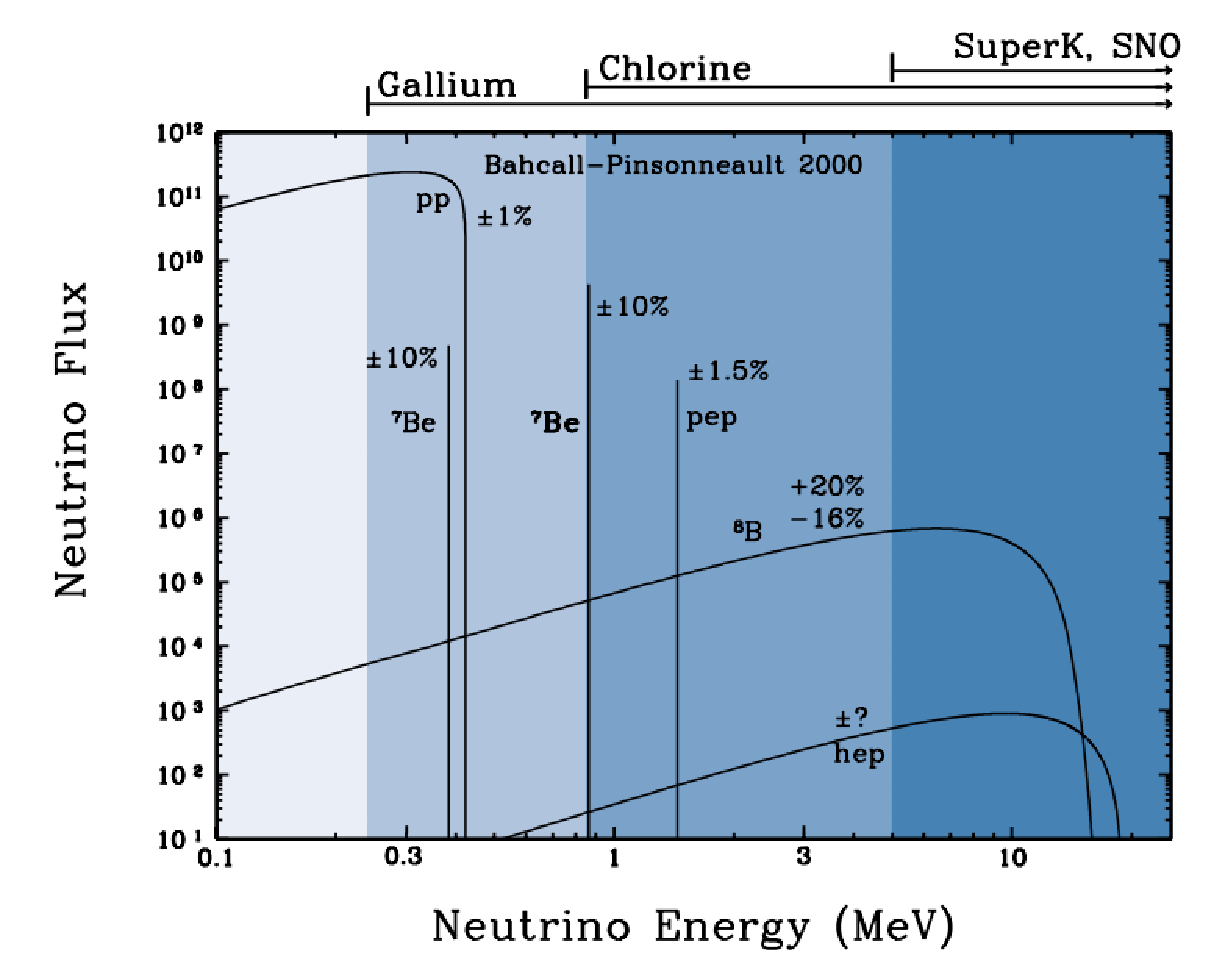
\includegraphics[width=\textwidth, trim={0mm 0mm 0mm 0mm}, clip,page=1]{Figures/Theory/SolarNeutrinoFlux.pdf}
  \end{subfigure}
  \caption{The solar neutrino flux as a function of neutrino energy for various fusion reaction and decay chains as predicted by the Standard Solar Model. Taken from \cite{Bellerive2004-ur}.}
  \label{fig:NeutrinoOscillationPhysics_SolarNeutrinoFlux}
\end{figure}

The first measurements of solar neutrinos observed a significant reduction in the event rate compared to predictions from the Standard Solar Model \cite{PhysRevLett.20.1205, Vinyoles2017-vv}. The proposed solution to this ``solar neutrino problem'' was \quickmath{\nu_{e} \leftrightarrow \nu_{\mu}} oscillations in a precursory version of the PMNS model \cite{Gribov1969-xi}. The Kamiokande \cite{PhysRevLett.63.16}, Gallex \cite{Hampel1999-of} and Sage \cite{PhysRevC.60.055801} experiments confirmed the \quickmath{\sim 0.5} deficit of solar neutrinos.

\subsection{Atmospheric Neutrinos}
\label{subsec:NeutrinoOscillationPhysics_AtmosphericNeutrinos}

\subsection{Accelerator Neutrinos}
\label{subsec:NeutrinoOscillationPhysics_AcceleratorNeutrinos}

\subsection{Reactor Neutrinos}
\label{subsec:NeutrinoOscillationPhysics_ReactorNeutrinos}

\section{Open Questions}
\label{sec:NeutrinoOscillationPhysics_OpenQuestions}
